%% BRANCH paper, HCAI 2026/2027, IJCAI-ECAI 26 format.
%% Build: latexmk -pdf main.tex   (or: bash reproduce.sh paper)
\documentclass{article}
\pdfpagewidth=8.5in
\pdfpageheight=11in
\usepackage{ijcai26}
\usepackage{times}
\usepackage{url}
\usepackage[hidelinks]{hyperref}
\usepackage[utf8]{inputenc}
\usepackage[small]{caption}
\usepackage{graphicx}
\usepackage{amsmath,amssymb,amsthm}
\usepackage{booktabs}
\usepackage{xcolor}
\usepackage[round,authoryear]{natbib}
\setcitestyle{aysep={}}           % Chicago author-date: (Sobol' 2001)
\urlstyle{same}

\newtheorem{proposition}{Proposition}
\makeatletter\newcommand{\tabinput}[1]{\@@input #1 }\makeatother
\newcommand{\repo}{\url{https://github.com/ashirabench/branch}}
\newcommand{\qFlipPriorOne}{1.41}
\newcommand{\qSobolPriorOne}{1.39}
\newcommand{\qEntPriorOne}{2.83}
\newcommand{\qRandPriorOne}{3.64}
\newcommand{\qMinPriorOne}{1.57}
\newcommand{\qFlipChosen}{2.87}
\newcommand{\qSobolChosen}{2.88}
\newcommand{\qEntChosen}{4.64}
\newcommand{\qRandChosen}{6.04}
\newcommand{\qFlipChosenTails}{2.61}
\newcommand{\qEntChosenTails}{3.93}
\newcommand{\wFlipTailsOne}{7.2\%}
\newcommand{\wFlipTailsTwo}{4.8\%}
\newcommand{\wFlipStrictTwo}{2.8\%}
\newcommand{\qFlipChosenTwo}{2.34}
\newcommand{\wFlipTailsStrictOne}{4.1\%}
\newcommand{\wFlipChosenTails}{1.7\%}
\newcommand{\wSobolTailsStrictOne}{3.3\%}
\newcommand{\wRandTailsOne}{5.2\%}
\newcommand{\wFlipPriorOne}{0.6\%}
\newcommand{\wFlipHoldThree}{2.6\%}
\newcommand{\wFlipHoldTwo}{3.9\%}
\newcommand{\qFlipHoldThree}{2.85}
\newcommand{\ciFlipTailsOne}{4.3--10.7\%}
\newcommand{\ciFlipChosenTails}{0.7--2.8\%}
\newcommand{\ciFlipStrictTwo}{1.5--4.1\%}
\newcommand{\ciFlipPriorOne}{0.0--1.1\%}
\newcommand{\ciFlipHoldThree}{1.1--4.4\%}
\newcommand{\ciFlipHoldTwo}{2.0--5.9\%}
\newcommand{\pSobolPriorOne}{1.000}
\newcommand{\pSobolChosen}{1.000}
\newcommand{\nRuns}{540}
\newcommand{\nCases}{18}
\newcommand{\nNoQLoose}{10}
\newcommand{\nNoQStrict}{6}
\newcommand{\nGridProducts}{166}
\newcommand{\nGridRegions}{83}
\newcommand{\nGrids}{81}
\newcommand{\maxDiffBench}{$3.7\times10^{-9}$}
\newcommand{\maxDiffGrids}{$1.1\times10^{-8}$}
\newcommand{\impCartonPT}{0.058}
\newcommand{\impCartonDE}{0.051}
\newcommand{\impCartonBR}{0.059}
\newcommand{\impPETPT}{0.109}
\newcommand{\impPETDE}{0.087}
\newcommand{\impPETBR}{0.100}
\newcommand{\impCanPT}{0.139}
\newcommand{\impCanDE}{0.139}
\newcommand{\impCanBR}{0.139}
\newcommand{\impGlassPT}{0.108}
\newcommand{\impGlassDE}{0.101}
\newcommand{\impGlassBR}{0.114}
\newcommand{\impGlassAM}{0.066}
\newcommand{\dropAM}{43\%}

% generated by experiments/proposal_assets.py
\newcommand{\pqClim}{2.87}
\newcommand{\pqEntClim}{4.64}
\newcommand{\pqRandClim}{6.04}
\newcommand{\pNoQClim}{6}
\newcommand{\pwClim}{0.2\%}
\newcommand{\pwTailsClim}{1.7\%}
\newcommand{\pwTailsCiClim}{0.7--2.8\%}
\newcommand{\pwCiClim}{0.0--0.6\%}
\newcommand{\pqAcid}{1.45}
\newcommand{\pqEntAcid}{2.22}
\newcommand{\pqRandAcid}{3.20}
\newcommand{\pNoQAcid}{12}
\newcommand{\pwAcid}{0.0\%}
\newcommand{\pwTailsAcid}{2.6\%}
\newcommand{\pwTailsCiAcid}{0.2--5.4\%}
\newcommand{\pwCiAcid}{0.0--0.7\%}
\newcommand{\pqWater}{1.34}
\newcommand{\pqEntWater}{2.33}
\newcommand{\pqRandWater}{3.56}
\newcommand{\pNoQWater}{12}
\newcommand{\pwWater}{0.0\%}
\newcommand{\pwTailsWater}{0.9\%}
\newcommand{\pwTailsCiWater}{0.0--2.6\%}
\newcommand{\pwCiWater}{0.0--0.7\%}
\newcommand{\pqFossil}{2.85}
\newcommand{\pqEntFossil}{4.46}
\newcommand{\pqRandFossil}{6.60}
\newcommand{\pNoQFossil}{6}
\newcommand{\pwFossil}{0.4\%}
\newcommand{\pwTailsFossil}{1.1\%}
\newcommand{\pwTailsCiFossil}{0.2--2.2\%}
\newcommand{\pwCiFossil}{0.0--0.9\%}
\newcommand{\pqNoLoc}{2.59}
\newcommand{\pqEntNoLoc}{4.07}
\newcommand{\pqRandNoLoc}{4.84}
\newcommand{\pNoQNoLoc}{9}
\newcommand{\pwNoLoc}{2.0\%}
\newcommand{\pwTailsNoLoc}{3.7\%}
\newcommand{\pwTailsCiNoLoc}{2.0--5.6\%}
\newcommand{\pwCiNoLoc}{1.1--3.1\%}
\newcommand{\pqUnif}{3.74}
\newcommand{\pqEntUnif}{5.24}
\newcommand{\pqRandUnif}{6.83}
\newcommand{\pNoQUnif}{6}
\newcommand{\pwUnif}{0.2\%}
\newcommand{\pwTailsUnif}{1.1\%}
\newcommand{\pwTailsCiUnif}{0.4--2.0\%}
\newcommand{\pwCiUnif}{0.0--0.6\%}


\title{Asking Only What Can Flip the Verdict: A Human-in-the-Loop BDI Agent\\
for Comparative Life Cycle Assessment}

\author{Ashira Benchimol
\affiliations
Department of Informatics Engineering, University of Coimbra, Portugal
}

\begin{document}
\maketitle

\begin{abstract}
Small companies are increasingly asked to compare the environmental footprint of the products they sell,
yet a comparative life cycle assessment (LCA) requires dozens of modelling choices that standards leave
to expert judgement. I built BRANCH to close this gap. BRANCH is a belief, desire, intention (BDI) agent
that uses no language model. It completes an LCA in openLCA from a bill of materials and a location, keeps
every unstated choice as an explicit random variable, and asks the human only the questions whose answer
can still reverse which product is better. Its query strategy scores a choice by the expected reduction of
$p(1-p)$, where $p$ is the probability that product A has the lower impact. This score is the value of
partial perfect information for the verdict under a quadratic loss; I note that it equals $p(1-p)$ times
the first-order Sobol index of the \emph{verdict}, which ties it to the sensitivity analysis LCA already
uses, and that the literal loss $\min(p,1-p)$ scores zero whenever no single answer can carry $p$ across
$1/2$. I tested BRANCH with simulated experts on \nCases{} cases built on real inventory data, which
compare four beverage packages in Portugal, Germany and Brazil with factors from the BAFU:2026 database.
With three questions per round and a 2.5\% certificate, BRANCH certifies the verdict with \qFlipChosen{}
questions on average, as few as a ranking by the Sobol index of the impact, the tool an LCA expert would
use, and 39\% fewer than uncertainty sampling (\qEntChosen{}), which cannot tell a decisive continuous
choice from an irrelevant one; random order needs \qRandChosen{}. When the expert answers from the agent's own
beliefs, at most 0.7\% of its certificates are wrong. The main empirical finding concerns the certificate. When the expert
answers from the tails of those beliefs, the strategy that asks the fewest questions is also the one that
certifies wrong verdicts most often, \wFlipTailsOne{} with one question per round and a 5\% certificate,
because it stops as soon as one answer seems to settle the matter; three questions per round bring the
share to \wFlipHoldThree{} (\ciFlipHoldThree{}) on new sessions. The method does not depend on the product:
packaging is the first domain with codified rules, and any other product can be described by processes chosen from the
database. The code is available at \repo.
\end{abstract}

%% ------------------------------------------------------------------
\section{Introduction}

Product level environmental information is moving from voluntary to mandatory. The European Packaging and
Packaging Waste Regulation \citep{ppwr2024}, the Product Environmental Footprint method \citep{zampori2019}
and the forthcoming digital product passport all ask companies for defensible, comparable numbers on the
life cycle of what they sell. Life cycle assessment (LCA) is the method behind those numbers
\citep{iso14040,iso14044}, and most of the companies concerned are small and medium enterprises (SMEs)
without an LCA expert.

The free and widely used tool openLCA reads every major inventory database and computes impacts. The
modelling choices stay with the user, and that is where a non-expert gets stuck. Before the first result appears the user must decide the functional
unit, the system boundary, the recycling rule, the recycled content, the number of trips of a refillable
container, the electricity mix, transport distances and which of several near identical datasets
represents a material \citep{ilcd2010}. Each choice is a branch in a tree; some branches reverse the
conclusion between two products and most do not. The same product can receive very different footprints
depending on boundary and allocation \citep{schmidt2009}, and whether capital goods are included matters
for some product groups and not for others \citep{frischknecht2007}. The difficulty for a non-expert is
not computing but choosing.

Current practice answers this with uncertainty and global sensitivity analysis. The analyst propagates
distributions by Monte Carlo and ranks inputs by their share of the variance of the result
\citep{heijungs2001,groen2017,igos2019}. For a
comparison, however, variance is not the right target. An input can be very uncertain and still never
change which product wins, while a modest input can decide the comparison \citep{mendoza2018}. Recent
systems use language model agents to automate parts or all of the assessment, from matching impact factors
to writing the report \citep[reviewed by][]{preuss2026}, for example from a product photo or name
\citep{zhang2026}, or let a practitioner build and calculate models in openLCA by conversation
\citep{below280_2026}. They take the modelling choices themselves or leave them to someone who can check
them; which few choices would change a given comparison, the question a non-expert most needs answered,
is not the question they address.

I take a third route, grounded in human-centred AI \citep{shneiderman2022}. BRANCH delegates the
routine choices to data and puts the human in the loop for the ones that matter. It is a BDI agent
\citep{rao1995,wooldridge2009} that receives a bill of materials and a location, holds a probability
distribution over every open modelling choice, and at each step decides whether to compute, to ask the
human one more question, or to certify the verdict. Which question to ask is an active learning problem
\citep{settles2009} in which the instance is a modelling choice and the label is the human's answer. The
agent picks the choice whose answer is expected to reduce the risk of a wrong verdict the most, in the
spirit of expected error reduction \citep{roy2001} and preposterior analysis \citep{howard1966,raiffa1961}.

The paper makes four contributions. First, I propose a query score for comparative decisions, the
expected reduction of $p(1-p)$, and note with a short identity that it equals $p(1-p)$ times the
first-order Sobol index of the verdict indicator. I also show that the literal loss $\min(p,1-p)$ scores
zero for every question whose answers all leave the verdict on the same side (Section~\ref{sec:lemma}).
Second, I test a stopping certificate against a simulated expert drawn from the tails of the agent's own
beliefs. With one question per round, the strategies that ask the fewest questions, decision flip among
them, make many wrong certificates. Third, I deliver a working, open-source companion for openLCA built on
real unit impact factors, with a web application and a report that states who decided each choice.
Fourth, I report a benchmark of \nCases{} comparisons built on real inventory data, with paired tests at
the level of cases against the uncertainty sampling strategies of active learning \citep{settles2009,faria2022}.

Section~\ref{sec:related} reviews related work,
Section~\ref{sec:materials} describes the data and tools, and Section~\ref{sec:methods} describes the
agent and the query strategy. Section~\ref{sec:experiments} presents the experiments and results,
Section~\ref{sec:discussion} discusses what they mean for human-centred AI, and
Section~\ref{sec:conclusions} concludes.

%% ------------------------------------------------------------------
\section{Related Work}\label{sec:related}

\paragraph{Uncertainty and sensitivity in LCA.}
ISO 14044 requires that comparative assertions address uncertainty and sensitivity \citep{iso14044}.
Data quality is usually scored with the pedigree matrix: each inventory value receives scores from 1 to 5
on reliability, completeness and temporal, geographical and technological representativeness, and each
score maps to an uncertainty factor that sets the spread of a lognormal distribution around the value
\citep{weidema2013}. Analysts then propagate the spreads and rank inputs by
perturbation or by Sobol indices of the result \citep{heijungs2001,sobol2001,saltelli2008,groen2017,igos2019}. \citet{mendoza2018} show that for comparative studies
the relevant quantity is the comparison itself, and propose indicators such as the share of Monte Carlo
runs in which one alternative beats the other. BRANCH builds on this view and goes one step further.
It uses the sensitivity of the comparison to decide what to ask a person, and it stops when the comparison
is settled.

\paragraph{Active learning and expected error reduction.}
Uncertainty sampling picks the instance whose label the model is least sure about (least confident,
margin, entropy), and expected error reduction picks the instance whose label is expected to reduce the
future error the most \citep{settles2009,roy2001}. Stopping rules end the loop once more labels are
unlikely to help \citep{vlachos2008}. \citet{faria2022} showed that query strategy and batch size jointly
determine how many labels are needed. BRANCH transfers these ideas from labelling data to eliciting
modelling choices. The person is the oracle, the open choices form the pool, the decision flip score is
expected error reduction applied to the verdict, the certificate is the stopping rule, and the rounds of
three questions are batch-mode active learning. BRANCH compares against the same uncertainty sampling
baselines (least confident, margin and entropy).

\paragraph{Value of information.}
Preposterior analysis computes the expected value of observing a variable before a decision
\citep{raiffa1961,howard1966}. In health economics, the expected value of partial perfect information
ranks parameters by how much learning them would improve a decision, and it is known to differ from
variance-based rankings of the outcome \citep{felli1998,oakley2004,strong2013}. The decision flip score is
the value of partial perfect information for a binary decision under a quadratic loss. That this value is
the main effect of the decision indicator is a known relation, and Proposition~\ref{prop:sobol} restates
it in the vocabulary of LCA. With the binary entropy as the loss, the
same score is the mutual information between the answer and the verdict \citep{lindley1956}, the
criterion behind Bayesian active learning by disagreement \citep{houlsby2011}.

\paragraph{BDI agents and human-centred AI.}
The BDI model separates what an agent believes, what it wants and what it is committed to doing
\citep{bratman1987,rao1995}, which makes its behaviour explainable step by step. Human centred AI asks
for high automation together with high human control \citep{shneiderman2022}, and interactive machine
learning puts the person inside the loop as a source of knowledge rather than a labeller of last resort
\citep{amershi2014}. \citet{munro2021} separates human-assisted machine learning, where people train or
correct a model, from machine-learning-assisted humans, where the model supports a task that stays with the
person; the HCAI course at Coimbra calls the first Human in the Loop and the second Machine in the Loop or
Human in Command. Cooperative AI frames the problem as agents that help humans reach better joint decisions
under uncertainty, with trust and interpretability still open \citep{dafoe2020}. BRANCH is built on the
first model. Its core is a human-in-the-loop active learning loop in which the person is the source of
knowledge: the agent chooses what to ask, each answer corrects its beliefs, and the loop runs until the
verdict is certified. Human in command enters only at three points that Section~\ref{sec:roles} lists:
the value-laden choices, the decision to stop, and the use of the verdict.

\paragraph{Automated LCA.}
Language model agents are now applied to LCA from several directions. \citet{preuss2026} review about
twenty agent frameworks for LCA, most of them built on language models and aimed at inventory data, impact
factor matching and interpretation, and propose designs for full automation in which people verify the
agents' work after they converge; the limitations they tabulate include hallucination, unstable answers
to the same prompt and the absence of error detection. \citet{zhang2026} produce footprints from a product
image or name with multimodal agents, and \citet{nouri2026} put a conversational layer over a
deterministic engine for early-stage building LCA, so that the model explains and the engine computes. Inside openLCA, the
\texttt{b280-olca-mcp} server \citep{below280_2026} exposes the IPC interface to an assistant, so that a
practitioner can explore, build, audit and calculate models by conversation.
BRANCH works on a different step of the same workflow: not how to build or explain a model by
conversation, but which of the open modelling choices a non-expert should be asked about, and when the
comparison can be certified. It also places the person differently: not as a verifier after the agents
have converged, but as the source of the few facts that decide the comparison, consulted while the
assessment is built. It contains no language model, so a person, or an assistant, can inspect
every belief, rule and source, and openLCA checks every result that BRANCH sends back. The two kinds of
tool are complementary: a conversational interface could collect the bill of materials and explain the
report, while BRANCH decides what to ask.

%% ------------------------------------------------------------------
\section{Materials}\label{sec:materials}

\paragraph{Inventory and impact method.}
All impacts come from the Life Cycle Inventory database of the Swiss Federal Administration, BAFU:2026
\citep{bafu2026}. I used it with the Environmental Footprint 3.1 method as adapted in that release and ran
both in openLCA 2.6. I chose this database because it is free, runs in openLCA and covers every
material, process and electricity grid the benchmark needs, so any SME can reproduce the results. I chose
EF~3.1 because it is the impact method of the European Product Environmental Footprint
\citep{zampori2019}. Its terms, however, forbid redistribution. The repository therefore
contains the extraction script and never the extracted factors. Every result BRANCH produces cites the
database.

\paragraph{Unit impact factors.}
LCA is linear in the amounts of each exchange. BRANCH therefore asks openLCA once, through its inter
process communication interface, for the impact of every candidate dataset per unit (kg of material, kWh
of electricity, tonne kilometre of transport, MJ of heat, kg of water) and stores it as a vector over all
16 EF~3.1 categories. The extraction for the benchmark covers 113 factors and leaves no dataset unresolved. These factors
describe six packaging materials (PET, HDPE, LDPE, glass, aluminium and liquid packaging board) with their
production and end of life processes, three transport modes, heat, water, three secondary packaging items
(corrugated box, stretch film and pallet) and 82 electricity grids, of which 81 are national or regional
and one is global. BRANCH computes every factor for one unit of the process's reference
exchange, for example 1 kWh, because it writes its amounts in that unit. Nine more packaging materials need
24 further factors, and the factor of any other process of the database is read when a person names it.

\paragraph{Regions.}
A region is a file that inherits from its parent (global, then country, then subregion). Each file states
the electricity mix, distribution distances and the priors of waste statistics, and tags every value with
its provenance (published source or assumption). For Portugal, Germany and Brazil the priors of recycling
rates, of the split between incineration and landfill and of recycled content come from national
statistics (Eurostat and the packaging reports of APA for Portugal, BMUV, GVM and ZSVR for Germany, ABIPET,
ABRALATAS, Tetra Pak and ABREMA for Brazil); trips, washing and distances remain assumptions. These
national priors entered the code on 4 November 2026, after the benchmark below was run with the catalogue
defaults, and I re-ran the whole benchmark on 13 November 2026 with the national priors, after the checks described below. The results below
come from that run; the repository keeps the earlier priors and their results as a snapshot. The code also ships subregions such as the Brazilian
state of Amazonas, where the electricity question (national grid or isolated oil system) and a river leg
in the supply chain become open choices.

\paragraph{Checks of the priors.}
For the choices that still rest on assumptions I looked for published values and read each one in its
original document. I use these values to check the priors and not to set them, because one case study does
not give the typical value of a country. The rule was fixed before I looked at any result: no most
probable value changes, no range becomes narrower, and a range is widened only when a published value
falls outside it. Ten values were compared: the mass of the 330~mL can \citep{mpe2022}, the mass of the 1~L
refillable glass bottle in Italy, Germany and Brazil \citep{tua2020,schonert2002,morini2019}, the mass of
the 1~L PET bottle and the trips of a pool bottle in Germany \citep{schonert2002}, the heat and the water
for washing and the distribution distance \citep{tua2020}, and the recycled content declared by one can
maker \citep{ardagh2021}. Eight lay inside their prior. Two lay outside, and I widened those two priors.
The heat for washing one bottle was measured as 0.459~MJ in an Italian bottling plant, against an upper
bound of 0.4, and the 1~L refillable bottle for soft drinks in Brazil weighs 950~g according to its
manufacturer, against an upper bound of 750. The electricity of the Italian plant, 44~Wh per bottle,
covers the whole plant and not only washing, so I did not compare it with the washing prior. The values
are in \texttt{data/prior\_checks.csv}, and a test fails when a prior excludes one of them. The widening
changed no verdict at the central values of the 18 cases, and all the results below use the widened priors;
the repository keeps the summaries from before the widening.

\paragraph{Benchmark products.}
The benchmark compares four beverage packages per litre delivered. They are a single-use PET bottle
(1 L), a refillable glass bottle (1 L), an aluminium can (330 mL) and an aseptic beverage carton (1 L).
I chose them because published comparative studies exist and the verdict is known to depend on trips,
recycling and distance. The six pairs in three regions give \nCases{} cases. Each case has between 11 and 21
open choices, 16 on average, which cover component masses, dataset grade, recycled content, collection
and incineration shares, trips, washing energy, heat and water, end of life route and distances.

\paragraph{Two ways to describe a product.}
The agent, its query score and its certificate know nothing about packaging. What is specific to a domain is how a
product becomes exchanges and open choices, and BRANCH offers two ways. For a container, the person gives a bill of
materials, and codified rules add forming, distribution, refill and end of life with labelled priors; this is the way
of the benchmark. For any other product, the person names processes of the database (11,951 in BAFU:2026) by life cycle
stage and gives an amount for each, or the smallest and the largest amount when it is not known. Each range becomes an
open choice with a uniform prior labelled as an assumption given by the user, and the agent asks for the exact amount
only if it can flip the verdict. The person also states the service both products deliver and how many of each are
needed for it. The two ways can be mixed in one product.

\paragraph{Tools.}
The engine runs in Python with NumPy and SciPy, and the olca-ipc and olca-schema packages connect it to
openLCA. Gradio serves the web application, ReportLab writes the PDF report and pytest runs 148 tests.
PyInstaller builds the desktop connector \emph{BRANCH for openLCA}, and Docker handles deployment. The
engine also runs unchanged on CuPy arrays.

%% ------------------------------------------------------------------
\section{Methods}\label{sec:methods}

\begin{figure*}[t]
\centering
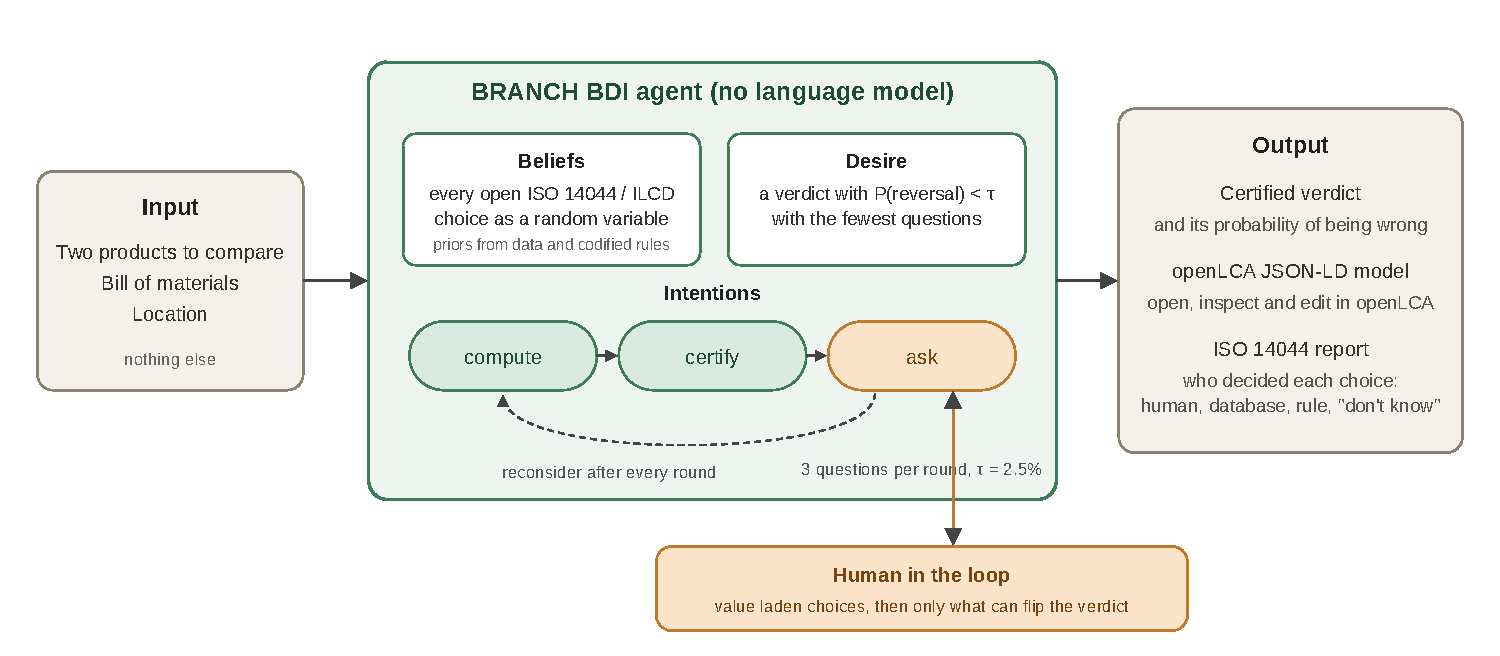
\includegraphics[width=0.86\textwidth]{figures/overview.pdf}
\caption{The bill of materials and the location fix the deterministic part of the beliefs, and every
remaining choice is a random variable. The agent computes, certifies or asks, and it reconsiders after
every round of answers.}
\label{fig:overview}
\end{figure*}

\subsection{Beliefs, desire and intentions}

Figure~\ref{fig:overview} shows the agent. Its \emph{beliefs} are a model with two alternatives A and B
and open choices $X=(X_1,\dots,X_J)$. A continuous choice (a mass, a share, a number of trips, a
distance) has a triangular, uniform, normal or lognormal prior; a categorical choice (which dataset, which
end of life route, which electricity system) has a probability vector. The impact of each alternative is
a sum of terms, each the product of an inventory amount that depends on the choices and a unit impact
factor, so $\Delta(X)=I_A(X)-I_B(X)$ is cheap to evaluate. The \emph{desire} is a verdict on the sign of
$\Delta$ whose probability of being wrong is below a threshold $\tau$, reached with as few questions as
possible. The \emph{intentions} follow the agent control loop of \citet{wooldridge2009}: each answer is a
percept that revises the beliefs (the function \texttt{brf}), the open choices are the options, the score
of Section~\ref{sec:lemma} is the filter that turns options into intentions, and the loop ends when the
intention has succeeded (the certificate holds) or has become impossible (nothing is left to ask). The
agent reconsiders its intentions after every round, as in the version of the loop with reconsideration.
The loop has four steps.
\begin{enumerate}
\item In the \textbf{compute} step, the agent draws $N=20{,}000$ samples of $X$ once (common random
numbers) and estimates $p=P(\Delta<0)$. With this $N$ the standard error of $p$ is at most 0.4
percentage points, well below the 2.5\% certificate, and each step still takes milliseconds.
\item In the \textbf{certify} step, the agent stops and reports if $\min(p,1-p)<\tau$.
\item In the \textbf{ask} step, the agent first asks the value-laden choices, such as whether capital
goods belong in the system boundary, which always stay with the human. Otherwise it scores every open choice and asks
the $b$ best, which form the batch. Ties keep the order of the model.
\item In the \textbf{reconsider} step, the agent fixes each answered choice to its value, or keeps its
prior if the answer is ``I don't know'', and returns to the first step.
\end{enumerate}
Conditioning on an answer only replaces one column of the sample matrix, so each step takes milliseconds
and the person never waits.

\paragraph{Where the human is.}\label{sec:roles}
The loop above is human in the loop in the sense of the course and of \citet{munro2021}: the agent
selects the queries, as in active learning, and the human answers them as the oracle, so the human is the
source of the knowledge that the data cannot give. This is the base of BRANCH, and the ask and reconsider
steps are where it happens. The human is in command, and the agent only assists, at three points. First,
the value-laden choices, such as the system boundary, are always asked and never scored or delegated to
the data. Second, the person can answer ``I don't know'', which keeps the prior, or finish the session at
any time, and the report then states the probability that the verdict is wrong. Third, the verdict is
advice: the person decides what to do with it, and a comparison meant for the public goes to the critical
review of ISO 14044. Every other choice is resolved by the human-in-the-loop process.

\subsection{The decision flip score}\label{sec:lemma}

Let $D=\mathbf{1}\{\Delta(X)<0\}$, so $p=E[D]$, and let $p_j(x)=P(D=1\mid X_j=x)$. The choices are
independent under the prior. A myopic strategy
scores choice $j$ by the expected reduction of a loss $g$ of the verdict probability,
\[
R_g(j)=g(p)-E_{X_j}\!\left[g\big(p_j(X_j)\big)\right],
\]
and by the law of total probability $E_{X_j}[p_j(X_j)]=p$.

\begin{proposition}\label{prop:sobol}
For $g(p)=p(1-p)$, $R_g(j)=\mathrm{Var}_{X_j}\!\left(E[D\mid X_j]\right)=p(1-p)\,S_j(D)$, where
$S_j(D)$ is the first-order Sobol index of the verdict indicator.
\end{proposition}
\begin{proof}
$R_g(j)=p-p^2-E[p_j-p_j^2]=E[p_j^2]-p^2=\mathrm{Var}(p_j)$ because $E[p_j]=p$. Since $D$ is Bernoulli,
$\mathrm{Var}(D)=p(1-p)$, and $S_j(D)=\mathrm{Var}(E[D\mid X_j])/\mathrm{Var}(D)$.
\end{proof}

The identity is elementary, and I claim it only as the bridge between the two literatures. Ranking by
$R_g$ is ranking by the share of the \emph{verdict's} variance each choice explains. Classical LCA
sensitivity ranks by $S_j(\Delta)$, the share of the variance of the \emph{result}, which can be large for
a choice that never changes which product wins.

\begin{proposition}\label{prop:stall}
For $m(p)=\min(p,1-p)$, if every answer to $j$ leaves the verdict on the same side ($p_j(x)\le 1/2$ for
all $x$ when $p\le 1/2$, or symmetrically), then $R_m(j)=0$.
\end{proposition}
\begin{proof}
For $p\le 1/2$ and $p_j\le 1/2$, $m(p_j)=p_j$, so $E[m(p_j)]=E[p_j]=p=m(p)$. The other case is symmetric.
\end{proof}

When the verdict leans one way but is not yet certified, often no single answer carries $p$ across
$1/2$. Every choice then scores zero under the literal loss, and the agent falls back on the order of the
model. The smooth loss is strictly concave, so $R_g(j)>0$ as soon as an answer moves $p$ at all.

\begin{proposition}\label{prop:bounds}
For every $p\in[0,1]$, $m(p)\le 2p(1-p)\le 2m(p)$.
\end{proposition}
\begin{proof}
For $p\le 1/2$, $m(p)=p$ and $1/2\le 1-p\le 1$. The case $p\ge 1/2$ is symmetric.
\end{proof}

The smooth loss therefore stays within a factor of two of the literal one, so it only changes which
question comes next. BRANCH still stops when $m(p)<\tau$, and $m(p)$ is the probability that the verdict
is wrong under the current beliefs.

\paragraph{Estimation.}
BRANCH represents the answers of a continuous choice by $K=5$ quantile points of equal weight (the
10th, 30th, 50th, 70th and 90th percentiles) and estimates every $p_j(x_k)$ from the same $N$ samples.
Five points cover the low, middle and high answers while keeping the cost at five conditional estimates
per choice. This gives two estimators of $R_g$. The plug-in
version (\texttt{decision\_flip}) uses the sample estimate of $p$ for the loss before the answer. The total
probability version (\texttt{decision\_flip\_tp}) uses $\bar p_j=\sum_k w_k p_j(x_k)$ and equals
$\bar p_j(1-\bar p_j)S_j(D)$ exactly. The ablation compares both estimators with the binary entropy of $p$,
another smooth loss, and with the literal loss. Unit tests check the three propositions and both
decompositions numerically.

\subsection{Baselines}

Three baselines come from active learning \citep{settles2009} and look at the answer probabilities
$\pi$ of each choice. \emph{Least confident} scores $1-\max_k \pi_k$, \emph{margin} scores the negative gap
between the two most probable answers, and \emph{entropy} scores the entropy of $\pi$. For a continuous
choice, $\pi$ gives equal weight to its five quantile answers, so every continuous choice gets the same
score, at least as high as any categorical one, and the ties keep the order of the model. Least confident and
entropy therefore rank the choices identically, and both ask the continuous choices, which dominate
these cases, in the order of the model. A fourth baseline asks in \emph{random} order. The fifth
comes from LCA \citep{saltelli2008,groen2017}. It ranks choices by the first-order \emph{Sobol} index of
$\Delta$, which BRANCH estimates from the same conditional samples. Sobol indices are the standard
global sensitivity measure in LCA \citep{groen2017}, so this is what an LCA expert would use to decide
which choice to examine first. It is the strongest and fairest rival, because beating only entropy and
random order would show little. All strategies share the same loop,
samples, certificate and stopping rule, so they differ only in which question comes next.

\subsection{Outputs and safeguards}

The report lists the verdict and its probability of being wrong, the impacts of both alternatives in all
16 EF~3.1 categories with a warning when they disagree, the share of the impact due to disposal, every
choice with who decided it (human, database, rule, or ``I don't know'') and its source, and the smallest
single change that would reverse the verdict. At the start the agent asks whether the comparison will be
disclosed to the public. If so, it states, and repeats in the report, that ISO 14044 requires a critical
review by an independent panel. BRANCH prepares the study for that review but does not replace it. BRANCH
can write the resolved model as openLCA JSON-LD or push it to a running openLCA, which recomputes it.

%% ------------------------------------------------------------------
\section{Experiments}\label{sec:experiments}

\subsection{Setup}

\paragraph{Simulated experts.}
For each case and seed, the simulation draws a hidden ``true'' value of every choice, and the expert
answers each question with it. The verdict at the true values serves as the reference. The experiments
use two expert models. In the
\emph{prior} model the simulation draws the truth from the agent's own priors, which tests efficiency when
the beliefs are right. In the \emph{tails} model it draws each truth from the outer 10\% of the prior (and never from
the most probable category), which tests the certificate when the beliefs are wrong in a way they do not
anticipate. I chose 10\% because the agent represents a continuous answer by its 10th to 90th
percentiles, so every true value then lies outside all the answers the agent considers, while it stays a
value the prior allows.

\paragraph{Design.}
The design crosses \nCases{} cases with 30 seeds, which gives \nRuns{} runs per strategy and batch size.
Following \citet{faria2022}, the batch size goes from 1 to 5. The certificate takes the values
$\tau=5\%$ and $\tau=2.5\%$. Climate change is the main indicator because it is the category that
companies are most often asked to report, and the report still gives all 16 categories. The outcome is the number of
questions until certification and whether the certified verdict agrees with the reference.

\paragraph{Statistics.}
The sessions of one case share its beliefs, so the unit of inference is the case, not the session.
Every strategy sees the same cases, seeds and simulated experts. I compare each strategy with
\texttt{decision\_flip} through its mean number of questions per case, with an exact paired sign-flip
permutation test over the \nCases{} cases and a Holm correction over the nine rival strategies of each batch size.
The 95\% intervals of the question savings and of the share of wrong certificates come from a bootstrap
over cases with 10,000 resamples. When no certificate is wrong, I give the exact binomial interval over
sessions, which ignores the clustering and is therefore optimistic. At $\tau=5\%$ the agent certifies
\nNoQLoose{} of the \nCases{} cases before any question, and at $\tau=2.5\%$ it certifies \nNoQStrict{}. Every strategy
ties on those cases, so the tests rest on 8 informative cases at $\tau=5\%$ and 11 at $\tau=2.5\%$. With 8
cases the smallest $p$ value the test can give is 0.008, which the Holm correction over nine strategies
turns into 0.070. At $\tau=5\%$ no difference can therefore reach the 5\% level after correction, however
large it is; at $\tau=2.5\%$ the smallest Holm-adjusted $p$ value is 0.009.

\paragraph{New seeds.}
I chose the batch size of the application on this benchmark. To check the choice, I ran 30 new seeds
(1000 to 1029) on the same \nCases{} cases with tail experts and $\tau=2.5\%$, for two and three questions
per round. These sessions played no part in the choice, but the cases are the same.

\paragraph{Reproducibility.}
A single command installs the environment, extracts the factors from a local openLCA, reruns every
experiment, regenerates every figure and table, and recompiles this paper (\texttt{bash reproduce.sh}).

\subsection{Results}

I report the benchmark that I ran after correcting the factors (see Agreement with openLCA).

\paragraph{Question efficiency.}
Figure~\ref{fig:batch} shows the mean number of questions with prior experts and $\tau=5\%$. With one
question per round, decision flip needs \qFlipPriorOne{} questions, entropy and least confident
\qEntPriorOne{}, and random \qRandPriorOne{} (raw $p=0.008$, the smallest value that 8 informative cases allow, and Holm-adjusted $p=0.070$). The uncertainty sampling
baselines look only at how spread the answers to a choice are, not at whether the choice matters. They
beat random order, but by a much smaller margin than decision flip does. Sobol of the impact comes close
(\qSobolPriorOne{}, $p=\pSobolPriorOne$), because in these cases the choices that dominate the variance of
$\Delta$ also tend to dominate the verdict. The gap of 0.01 questions has a bootstrap interval of $-0.06$ to
0.07. No interval at any batch size lies clearly above zero, and no batch size survives the Holm
correction.

\begin{figure}[t]
\centering
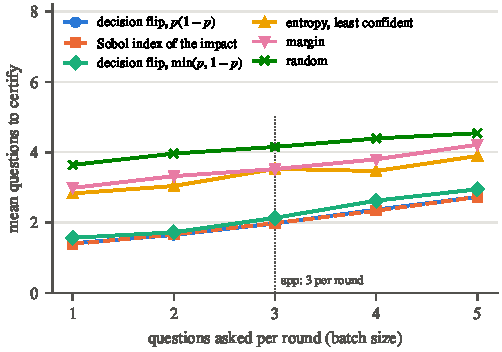
\includegraphics[width=\columnwidth]{figures/batch.pdf}
\caption{The mean number of questions to certify grows with the batch size. The experts answer from the
priors with $\tau=5\%$, each point pools \nRuns{} runs, Least confident coincides with entropy, and the
dotted line marks the three questions per round of the application.}
\label{fig:batch}
\end{figure}

\paragraph{The literal loss is less efficient.}
As Proposition~\ref{prop:stall} suggests, with prior experts the plug-in estimate of $\min(p,1-p)$ asks
more questions at every batch size (\qMinPriorOne{} against \qFlipPriorOne{} at batch 1), because it often scores every choice near zero and Monte Carlo noise then picks the question. Its total
probability estimate, which scores exactly zero in that situation and falls back on the order of the
model, does worse still (2.21 questions). After the Holm correction the difference between the literal
loss and $p(1-p)$ is significant at $\tau=2.5\%$ for four of the five batch sizes with prior experts, and
at $\tau=5\%$ for none, where only 8 cases are informative. With tail experts the gap in questions is of similar
size, and it is significant in two of the six conditions (Table~\ref{tab:losses}). At one and two
questions per round, the three smooth losses (plug-in, total probability, binary entropy) differ by at
most 0.05 questions. At three questions per round with tail experts and $\tau=2.5\%$, the total
probability version asks fewer questions than the plug-in version (2.42 against 2.49, $p=0.38$), but
2.2\% of its certificates are wrong against 1.9\%. Neither the total probability version nor the binary
entropy version differs significantly from the plug-in version in any of the twelve conditions after the
Holm correction. I keep the plug-in version as the default because the gains are small and the run with
new seeds checks the plug-in version.

\begin{table*}[t]
\centering
\small
\setlength{\tabcolsep}{4pt}
\begin{tabular}{lcccccccccccc}
\toprule
& \multicolumn{3}{c}{Priors 5\%} & \multicolumn{3}{c}{Priors 2.5\%} & \multicolumn{3}{c}{Tails 5\%} &
\multicolumn{3}{c}{Tails 2.5\%}\\
Loss & $b{=}1$ & $2$ & $3$ & $b{=}1$ & $2$ & $3$ & $b{=}1$ & $2$ & $3$ & $b{=}1$ & $2$ & $3$\\
\midrule
\tabinput{tables/losses.tex}
\bottomrule
\end{tabular}
\caption{Each cell gives the mean number of questions to certify for one loss, expert model, certificate
and batch size $b$. Every row except the total probability one uses the plug-in estimate, and an asterisk marks a
Holm-adjusted case-level $p<0.05$ against $p(1-p)$.}
\label{tab:losses}
\end{table*}

\paragraph{Calibration under wrong beliefs.}
With prior experts, decision flip is calibrated. At most 0.7\% of its certified verdicts are
wrong at either certificate and any batch size (interval 0.2--1.5\%). No strategy exceeds 1.2\% in any
setting with prior experts. With tail experts the picture changes (Figure~\ref{fig:calibration}). With
one question per round, \wFlipTailsOne{} of certified verdicts are wrong (\ciFlipTailsOne{}), which exceeds
the 5\% target. Random order still reaches \wRandTailsOne{}, so wrong beliefs alone bring the error to about the
target, and stopping after a single question adds the rest. Tightening the certificate to 2.5\% alone does not fix it
(\wFlipTailsStrictOne{}). Decision flip finds the one question that seems to settle the verdict and stops,
which is exactly what fails when the beliefs about the remaining choices are wrong. At $\tau=2.5\%$, two
questions per round give \wFlipStrictTwo{} (\ciFlipStrictTwo{}) and three give \wFlipChosenTails{}
(\ciFlipChosenTails{}), and four or five keep the share below 1\%. The share falls as the batch
grows, so three is not an isolated good value. On the new seeds, three questions per round give
\wFlipHoldThree{} (\ciFlipHoldThree{}) and two give \wFlipHoldTwo{} (\ciFlipHoldTwo{}). With two questions
per round the point estimate exceeds the target; with three it stays below it, although the intervals
overlap. I keep three, at a cost of about half a question. The data cannot rule out rates up to 4.6\% for
three questions per round. The new seeds give a higher share than the 1.9\% of the benchmark, as one
expects from a value chosen on the same data, so \wFlipHoldThree{} is the figure I report.

\begin{figure}[t]
\centering
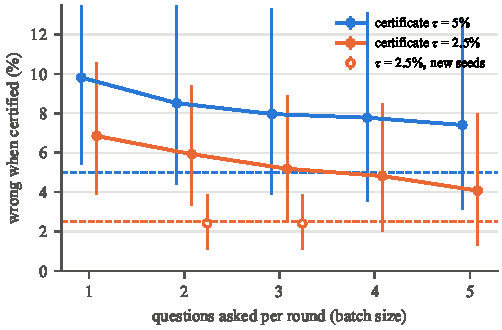
\includegraphics[width=\columnwidth]{figures/calibration.pdf}
\caption{The share of certified verdicts that are wrong falls as decision flip asks more questions per
round, with experts answering from the tails. The bars show 95\% intervals from a bootstrap over cases, the
dashed lines show the certificate $\tau$, and the hollow markers show the run with new seeds.}
\label{fig:calibration}
\end{figure}

\paragraph{Chosen setting.}
The web application therefore uses $\tau=2.5\%$ and three questions per round. Table~\ref{tab:main} gives
every strategy in this setting under both expert models. With prior experts, decision flip needs
\qFlipChosen{} questions, against \qEntChosen{} for entropy and \qRandChosen{} at random, 39\% fewer
than uncertainty sampling and less than half of random order. It ties with the Sobol index of the impact
(\qSobolChosen{}, $p=\pSobolChosen$). Robustness costs about 1.3 questions compared with the
most aggressive setting ($\tau=5\%$ and one question per round, \qFlipPriorOne{} questions), and about half
a question compared with two questions per round (\qFlipChosenTwo{}).

\begin{table*}[t]
\centering
\small
\setlength{\tabcolsep}{8pt}
\begin{tabular}{lcccccc}
\toprule
& \multicolumn{3}{c}{Experts from priors} & \multicolumn{3}{c}{Experts from tails}\\
Strategy & $Q$ & $p$ & W\% & $Q$ & $p$ & W\% \\
\midrule
\tabinput{tables/main.tex}
\bottomrule
\end{tabular}
\caption{The strategies compared in the chosen setting ($\tau=2.5\%$, three questions per round). $Q$ is
the mean number of questions to certify, $p$ is the Holm-adjusted case-level permutation $p$ value against
decision flip, and W\% is the share of certified verdicts that are wrong. Each cell pools \nRuns{} runs.
The tails columns come from the runs used to choose the setting, and the new seeds give \wFlipHoldThree{} for
decision flip.}
\label{tab:main}
\end{table*}

\subsection{Other impact categories and knowledge ablations}\label{sec:proposal}

The proposal also promised results beyond climate change and ablations of the agent's knowledge. I fixed
both runs in a file of the repository before any of them existed (\texttt{experiments/PLAN\_2026-11-13.md}):
the chosen setting, seeds 0 to 29, both expert models and four strategies. I report them as descriptive,
without new tests, because the cases are the same \nCases{} and so the runs are not independent evidence.
Before the runs, the new code path reproduced the climate change summaries of Table~\ref{tab:main} exactly.
Table~\ref{tab:proposal} gives the results.

\begin{table*}[t]
\centering
\small
\setlength{\tabcolsep}{6pt}
\begin{tabular}{lccccccc}
\toprule
& & \multicolumn{4}{c}{$Q$, experts from priors} & \multicolumn{2}{c}{W\% of decision flip}\\
Run & $N_0$ & Decision flip & Sobol & Entropy & Random & Priors & Tails \\
\midrule
\tabinput{tables/proposal.tex}
\bottomrule
\end{tabular}
\caption{The chosen setting ($\tau=2.5\%$, three questions per round, seeds 0 to 29) in three other impact
categories and with knowledge removed from the agent. $N_0$ is the number of the \nCases{} cases certified
from the priors alone, $Q$ is the mean number of questions to certify and W\% is the share of certified
verdicts that are wrong, with the 95\% interval of a bootstrap over cases (exact binomial when none is
wrong). The first row repeats the climate change runs of Table~\ref{tab:main} on the same seeds. In the last
two rows the verdict is for climate change, and the expert and the reference verdict come from the national
model.}
\label{tab:proposal}
\end{table*}

\paragraph{Other impact categories.}
The order of the strategies is the same in acidification, water use and fossil resource use as in climate
change: decision flip and Sobol tie, entropy needs more questions and random order the most. Acidification
and water use are easier than climate change, since \pNoQAcid{} of the \nCases{} cases need no question,
so only six cases inform those rows. With experts from the tails, the share of wrong certificates is
\pwTailsWater{} for water use and \pwTailsFossil{} for fossil resources, but \pwTailsAcid{}
(\pwTailsCiAcid{}) for acidification, slightly above the 2.5\% target. The setting was chosen on climate
change, so these rows test it on outcomes it was not tuned on, and it holds in two of the three.

\paragraph{Knowledge ablations.}
Without the location, the agent uses the global electricity mix and the default priors, while the expert
answers with national values, which fall outside the default range for some choices. The agent does not ask
more (\pqNoLoc{} questions against \pqClim{}), but it is wrong more often: \pwNoLoc{} of its certificates
(\pwCiNoLoc{}) with experts from the priors, against \pwClim{} with the national model, and \pwTailsNoLoc{}
(\pwTailsCiNoLoc{}) with experts from the tails, above the target. With uniform priors over the national
ranges, the agent asks about one question more (\pqUnif{} against \pqClim{}) and is not wrong more often
(\pwUnif{} and \pwTailsUnif{}). In these cases the location therefore buys correct certificates, and the
shape of the priors buys about one question. The first ablation removes the electricity mix and the national
priors together, so it cannot say which of the two matters more, and neither comparison was tested. The third ablation of the proposal, the pedigree spreads,
cannot be run because BRANCH does not implement them. The global electricity mix used here is the one
grid that the validation against openLCA does not cover in a product system; only its unit was audited.

\subsection{Validation of the product}\label{sec:validation}

The benchmark above evaluates the query strategy. This subsection asks three questions about the product
itself: whether it computes what openLCA computes, whether its answers agree with published studies, and
whether a person can use it.

\paragraph{Agreement with openLCA.}
For every benchmark case, BRANCH pushed the model resolved at the median of each continuous choice and
the most probable option of each categorical one to openLCA. I ran this check on 13 November 2026 with the
national priors. openLCA then built and calculated the two product systems with its own linking and the EF~3.1
method. Over the 36 products of the \nCases{} cases, the largest relative difference between openLCA and
BRANCH for climate change was \maxDiffBench{}. The surrogate therefore reproduces openLCA to numerical
precision for these products. The check was not a formality. Its first run found a 2.3\% gap for the refillable glass bottle.
Checking each exchange alone in openLCA traced the gap to electricity. The extraction had computed that
factor per MJ, the unit of the flow, while BRANCH multiplied it by kWh, the unit of the exchange. Since the
fix, the extraction computes every factor per unit of the reference exchange, and the validation script runs with
the experiments (\texttt{experiments/validate\_openlca.py}). Because that error lived in a single dataset, I then
audited the reference unit of all 113 factors, which found no problem, and validated one comparison
(refillable glass against aluminium can) in each of the \nGrids{} national and regional grids and in two
Brazilian regions. Over these \nGridProducts{} products the largest relative difference was
\maxDiffGrids{}. No region uses the global grid, so I could not check it this way. On 14 November 2026 I added nine
materials and extracted the 24 factors they need, all per kg. For each of their 14 dataset options I pushed an example
product to openLCA in Portugal, Germany and Brazil. Over these 42 products the largest relative difference was
$6.7\times10^{-9}$ (\texttt{experiments/validate\_materials.py}). The same day I checked the second way of describing
a product with two shopping bags that are not containers, a cotton bag and a polypropylene bag, each described by
processes named in the database (fabric or granulate, forming, sea freight and disposal). openLCA and BRANCH
differ by at most $4.7\times10^{-10}$ for the two products, and three processes read by name gave exactly the factors
of the same processes read through the catalogue.

\paragraph{Agreement with published studies.}
With every choice resolved in the same way (the median of the trips prior, 19 in Portugal and Brazil and 34
in Germany, and 225~km), the beverage carton has the lowest climate impact in the three countries
(\impCartonPT{}~kg CO$_2$ eq per litre in Portugal, \impCartonDE{} in Germany and \impCartonBR{} in Brazil)
and the aluminium can the highest (\impCanPT{} in all three). The order of the middle pair
depends on the country. In Portugal refillable glass (\impGlassPT{}) stays ahead of single-use PET
(\impPETPT{}). In Germany and in Brazil single-use PET is ahead (\impPETDE{} against \impGlassDE{}, and \impPETBR{}
against \impGlassBR{}); the national priors give PET bottles a higher recycling
rate in these two countries than in Portugal, and in Brazil the prior of the bottle mass reaches 950~g. A review of comparative
studies of reusable bottles \citep{furberg2021} reports that aseptic cartons are often among
the best options, that refillable glass overtakes single-use PET after a few trips on short routes, and that long
distribution distances can reverse that comparison. The review identifies trips and distribution distance
as decisive, and both are open choices that BRANCH asks about when their answer can move the verdict. In Amazonas, where the bottle travels a short distance and
the supply arrives by river, the impact of the refillable bottle falls by about \dropAM{} (\impGlassAM{}). The agreement with the review concerns the
position of the carton and the drivers of the comparison between glass and PET. Absolute values differ between studies, because databases, system boundaries and
allocation rules differ.

\paragraph{The application.}
Of the 148 automated tests, 15 cover the web application, and most of them run it as a person would use it. They check that a full
session produces the manager report and the technical report, that ``finish now'' closes the session on
the current beliefs, that two skipped questions in a row bring the suggestion to finish, that an answer
outside the possible range is refused in plain words, and that every question carries a plain language
explanation. They also check the connection panel, which lists the four steps before the first comparison
(openLCA open with its IPC server, a database open, the BAFU:2026 database with EF~3.1, the factors read)
and names the next one to do. A further check uses the whole application with a real openLCA, through the same web
interface as the browser (\texttt{experiments/check\_app\_with\_openlca.py}). On 14 November 2026 it searched the database, filled
the form with the two shopping bags, pressed Compare, after which the application read the factors of six processes
from openLCA by itself, answered one of seven questions and skipped the others, opened both reports and sent the comparison to openLCA,
where the two products differed from BRANCH by at most $3.8\times10^{-8}$\%. GitHub Actions builds the installers for macOS and Windows and checks that each built
application starts, shows its version and completes one whole comparison up to the manager report. These tests show that the application works as designed. They do
not show that a manager understands the questions or trusts the report, because no person outside the
project has used it yet, and that is the main gap of this validation.

%% ------------------------------------------------------------------
\section{Discussion}\label{sec:discussion}

\paragraph{What the human is asked.}
The baselines from active learning ask about the choices whose answers are most spread. Every continuous
choice looks equally spread to them, so they ask continuous choices in the order of the model, whether or
not they move the result. Decision flip asks about a choice only when its answer can move the
verdict, whatever its type. This is the human-centred point of the work, because a person's
attention is the scarce resource.

\paragraph{Efficiency and fragility.}
The calibration result is a warning that may generalise beyond LCA. A myopic value of information
strategy is efficient precisely because it stops as soon as the beliefs say the matter is settled. When the
beliefs are wrong, its certificates inherit the error. Batching is a simple remedy. It forces the agent to
hear from the human on more than one choice before it trusts its own model of the rest.

\paragraph{Trustworthiness.}
BRANCH contains no language model: every number comes from a dataset or a stated rule, and every choice has an owner. The person
can answer ``I don't know'' or stop at any time, value laden choices are never delegated, and comparisons meant for the public
carry the ISO 14044 notice. These properties map onto the requirements of human agency and oversight,
transparency and accountability for trustworthy AI \citep{hleg2019}.

\paragraph{Ethics.}
A comparison that a company publishes becomes an environmental claim about its product. A certificate from
BRANCH says that the verdict is unlikely to be wrong under its beliefs and the answers it received, not
that the product is better in the world. A company could also answer the value-laden questions in its own
favour. BRANCH cannot prevent this, so it records who answered each question and states in the report that
a public comparison needs the critical review of ISO 14044 \citep{iso14044}.

\paragraph{What BRANCH offers a small company.}
In openLCA, a person who compares two packages must find and link every dataset and decide every quantity
before the first result appears. In the benchmark this means 10 to 21 exchanges per comparison (15.7 on
average) and 11 to 21 open choices (16 on average). BRANCH takes a bill of materials and a region, fills
every exchange from the database and gives every open choice a labelled prior. In the chosen setting it
then asks \qFlipChosen{} questions on average before it certifies, and \nNoQStrict{} of the \nCases{}
cases need no question. The person does not decide the other choices. They stay as distributions, and the
report lists each one with its source or with the word assumption, so the company sees what the verdict
rests on. The company also keeps the work. BRANCH writes both product systems into the company's own
openLCA database with one parameter per choice, so a consultant or a reviewer can open, check and extend
the model there. The manager receives a PDF in plain language, and the technical report gives all 16
impact categories. The code is free under MPL~2.0 and the database is free of charge. There are two ways to use it. With the desktop connector, the person installs openLCA and the database once, and the connection panel
guides the four steps. With the hosted application, one host (a consultant, an association or a university) extracts the factors once, and the
company needs only a browser. The code for hosting is in the repository, but no public instance exists: the terms of the database forbid redistribution,
and I have not confirmed that they allow a hosted calculator. This is what I
bring: a way to reach a first comparative result in openLCA at the cost of about three answers, with every
default made visible. I can state this capability and its cost in questions. I cannot yet state that it
helps a real company, because no person outside the project has used it. Three limits bound the claim today.
The catalogue holds 15 packaging materials: the six of the benchmark and nine added as data files
(corrugated board, cartonboard, kraft paper, polypropylene, polystyrene, expanded polystyrene, PVC, PLA and steel sheet).
No benchmark case uses the nine. Their computation agrees with openLCA (Section~\ref{sec:validation}), but their recycling rates are
assumptions, except for polypropylene and, in Germany, for paper, board and steel. Steel sheet stands for tinplate without its tin coating, and the expansion of
polystyrene beads is not modelled. For a product that is not a container there are no codified rules and no sourced priors:
the person chooses the processes and gives the ranges, and the amounts are treated as independent, so a mass and its
disposal are two separate questions. This way is checked against openLCA but is not part of the benchmark. Only Portugal, Germany and Brazil have priors from national statistics,
and even there about half of the open choices of a case rest on assumptions (8 of 16 on average). A company in
any other of the \nGrids{} electricity grids of the database can run BRANCH, but with default priors: for PET
against refillable glass in France, 12 of the 14 open choices are assumptions. The certificate was chosen on climate change, and in one of three other categories it missed its target
with experts from the tails (Section~\ref{sec:proposal}).

\paragraph{What changed since the proposal.}
The proposal of October 2026 fixed the commitments of this project, and the work departed from it in nine
ways. First, the proposal scored a question by the expected reduction of $\min(p,1-p)$. The agent stalled
with that loss (Section~\ref{sec:lemma}), so I replaced it with $p(1-p)$. Second, the proposal named the
Environmental Footprint reference package as the database. It was not available to me free of charge in openLCA format, so I used BAFU:2026. Third, the proposal asked one question per round and certified at 95\%. The
test with experts from the tails showed \wFlipTailsOne{} wrong certificates in that setting, so the chosen
setting asks three questions per round with $\tau=2.5\%$, and I confirmed it on new seeds. Fourth, the
proposal planned Wilcoxon tests. The sessions of one case are not independent, so I test at the level of
cases with a permutation test and a Holm correction, and I added the Sobol index of the impact as a
baseline. Fifth, the proposal planned reference models built by hand in openLCA. Instead BRANCH writes each
model into openLCA and openLCA recalculates it. This checks the computation, and it found the unit error
described in Section~\ref{sec:validation}, but it does not check the modelling, which the comparison
with published studies covers only in part. Sixth, the priors for recycling and disposal now come from national
statistics, and a check against ten published values widened two ranges. Spreads from the pedigree matrix
are not implemented. Seventh, two planned parts are missing: the study with five to seven participants and the ablation of the
pedigree spreads. The other impact categories and the other two knowledge ablations were run late, on a plan
fixed beforehand (Section~\ref{sec:proposal}). Eighth, the title of the proposal kept the human in command. The
course's terms fit the system better: the human in the loop is the base, and the human is in command at
three points (Section~\ref{sec:roles}). Ninth, the proposal named packaging as the benchmark, not as the scope. After the benchmark I added the second way of
describing a product, so that the agent serves any comparison whose processes are in the database. The main difficulty was that a strategy can look efficient and be
unsafe at once, and only the test built to make the certificate fail showed it.

\paragraph{Limitations.}
The simulated experts are not people. They answer every question with the true value, whereas a person
may misremember a distance or guess a share \citep{ohagan2006}, so the results say nothing yet about real
users. The benchmark covers four products and three regions, its tests concern climate change only, and only 8 to 11 of its
cases are informative. The runs in three other impact categories and the two ablations reuse the same cases and are descriptive. The run with new seeds reuses the same cases. The priors treat the choices as
independent; the recycling and disposal priors come from national statistics, but the component masses, the trips outside Germany, washing, the distribution distance, the recycled content of aluminium and, in Brazil, of PET, and the burden of recycled PET still rest on
assumptions, which every report marks. The strategy is myopic. The benchmark
cases contain no value-laden choice, so $Q$ leaves out the questions a person would answer about scope. The surrogate is
linear in the unit factors, which holds for attributional studies under ILCD Situation A
\citep{ilcd2010} but not for consequential ones. Datasets with a single value carry no uncertainty yet,
and the pedigree matrix \citep{weidema2013} is the natural next step. The benchmark is easy: 7 to 10 of
the 18 cases are decided by the priors alone, and the advantage that the theory predicts for the verdict
score over the impact score, for choices that move the result without moving the verdict, did not arise in
these cases.

%% ------------------------------------------------------------------
\section{Conclusions and Future Work}\label{sec:conclusions}

I presented BRANCH, a BDI agent that completes a comparative LCA from a bill of materials and a location
and asks the human only what can flip the verdict. Its query score is the expected reduction of
$p(1-p)$, which equals the Sobol index of the verdict scaled by $p(1-p)$, while the literal error
probability often scores every question zero. On \nCases{} cases built on real inventory data, with prior
experts and in the chosen setting, it certifies the verdict with as few questions as the Sobol index of
the impact, 39\% fewer than uncertainty sampling and less than half as many as random order. With experts drawn from the tails of its beliefs,
\wFlipHoldThree{} of its certificates are wrong on new seeds, below the 2.5\% target as a point estimate.
In three other impact categories the order of the strategies is the same, and the certificate keeps its
target in two of them. Without the location the agent asks no more questions but certifies wrongly more often.
Its results agree with openLCA to \maxDiffGrids{} in all \nGrids{} national and regional grids of the
database and in two Brazilian regions.

Future work includes a study with SME managers and LCA practitioners, experts who answer with error,
codified rules and sourced priors for domains beyond packaging, more regions and impact categories in the benchmark, a non-myopic strategy that looks two questions ahead,
secondary packaging in the bill of materials, uncertainty for single-value datasets and integration closer
to openLCA, as a contribution to olca-app under its MPL 2.0 licence.

\paragraph{Code and data.}
The repository \repo{} holds the software, the tests, the benchmark summaries, the validation
tables and the desktop connector \emph{BRANCH for openLCA}. All impact data come from the Life Cycle
Inventory database of the Swiss Federal Administration, BAFU:2026, and each user extracts the factors
from their own openLCA.

\paragraph{Use of AI tools.}
I used Claude Code (Anthropic) to write and revise code and text under my direction, as the course
allows. I defined the problem, made the design decisions, ran the factor extraction and every validation
in openLCA, reviewed every change before it entered the repository, and read every reference cited in
this text and checked it against its source.

% Chicago author-date reference list (Chicago Manual of Style, 17th ed.).
% Kept by hand so the style is exactly Chicago; cite with \citep / \citet (natbib).
\begin{thebibliography}{99}
\small

\bibitem[{Amershi et~al.(2014)}]{amershi2014}
Amershi, Saleema, Maya Cakmak, William Bradley Knox, and Todd Kulesza. 2014. ``Power to the People: The Role of Humans in Interactive Machine Learning.'' \emph{AI Magazine} 35 (4): 105--20.

\bibitem[{Ardagh Metal Packaging(n.d.)}]{ardagh2021}
Ardagh Metal Packaging. n.d. \emph{Ardagh Metal Packaging -- Europe Statement of Recycled Content for Fiscal Year 2021}. Luxembourg: Ardagh Metal Packaging.

\bibitem[{BAFU(2026)}]{bafu2026}
BAFU (Federal Office for the Environment). 2026. \emph{Life Cycle Inventory Database of the Swiss Federal Administration, BAFU:2026}. Version 1.1. Bern: Federal Office for the Environment. Distributed via openLCA Nexus. \url{https://www.bafu.admin.ch/de/oekobilanzierung}. Accessed October 2026.

\bibitem[{Below280(2026)}]{below280_2026}
Below280 Limited. 2026. \emph{b280-olca-mcp: MCP Server Connecting AI Assistants to openLCA via Its IPC Server}. Version 1.16.0. Python package. \url{https://pypi.org/project/b280-olca-mcp/}. Accessed 4 November 2026.

\bibitem[{Bratman(1987)}]{bratman1987}
Bratman, Michael E. 1987. \emph{Intention, Plans, and Practical Reason}. Cambridge, MA: Harvard University Press.

\bibitem[{Dafoe et~al.(2020)}]{dafoe2020}
Dafoe, Allan, Edward Hughes, Yoram Bachrach, Tantum Collins, Kevin R. McKee, Joel Z. Leibo, Kate Larson, and Thore Graepel. 2020. ``Open Problems in Cooperative AI.'' arXiv preprint arXiv:2012.08630. \url{https://arxiv.org/abs/2012.08630}.

\bibitem[{European Commission(2010)}]{ilcd2010}
European Commission, Joint Research Centre, Institute for Environment and Sustainability. 2010. \emph{International Reference Life Cycle Data System (ILCD) Handbook: General Guide for Life Cycle Assessment, Detailed Guidance}. EUR 24708 EN. Luxembourg: Publications Office of the European Union.

\bibitem[{European Commission(2020)}]{annexc2020}
European Commission. 2020. \emph{Part C of Annex II (Former Annex C): List of Default CFF Parameters, Version 2.1, May 2020}. Brussels: European Commission.

\bibitem[{European Parliament and Council(2024)}]{ppwr2024}
European Parliament and Council. 2024. ``Regulation (EU) 2025/40 of 19 December 2024 on Packaging and Packaging Waste.'' \emph{Official Journal of the European Union} L, 22 January 2025. \url{https://data.europa.eu/eli/reg/2025/40/oj}.

\bibitem[{Faria et~al.(2022)}]{faria2022}
Faria, Bruno, Dylan Perdig\~ao, Joana Br\'as, and Lu\'is Macedo. 2022. ``The Joint Role of Batch Size and Query Strategy in Active Learning-Based Prediction: A Case Study in the Heart Attack Domain.'' In \emph{Progress in Artificial Intelligence: 21st EPIA Conference on Artificial Intelligence, EPIA 2022}, edited by Goreti Marreiros, Bruno Martins, Ana Paiva, Bernardete Ribeiro, and Alberto Sardinha. Lecture Notes in Artificial Intelligence 13566. Cham: Springer. \url{https://doi.org/10.1007/978-3-031-16474-3_38}.

\bibitem[{Felli and Hazen(1998)}]{felli1998}
Felli, James C., and Gordon B. Hazen. 1998. ``Sensitivity Analysis and the Expected Value of Perfect Information.'' \emph{Medical Decision Making} 18 (1): 95--109.

\bibitem[{Frischknecht et~al.(2007)}]{frischknecht2007}
Frischknecht, Rolf, Hans-J\"org Althaus, Christian Bauer, Gabor Doka, Thomas Heck, Niels Jungbluth, Daniel Kellenberger, and Thomas Nemecek. 2007. ``The Environmental Relevance of Capital Goods in Life Cycle Assessments of Products and Services.'' \emph{International Journal of Life Cycle Assessment} 12 (Special Issue 1): 7--17.

\bibitem[{Furberg et~al.(2021)}]{furberg2021}
Furberg, Anna, Astrid Lye Moum, Sander N{\o}rsterud, and Hanne Lerche Raadal. 2021. \emph{Review of Life Cycle Assessments of Reuse Systems for Bottles}. Report OR.37.21. Fredrikstad: NORSUS Norwegian Institute for Sustainability Research.

\bibitem[{GreenDelta(2022)}]{elcd2022}
GreenDelta. 2022. \emph{ELCD 3.2 Database for openLCA, Version 2.18, Correction of 8 September 2022}. Data of the European Commission, Joint Research Centre. Berlin: GreenDelta.

\bibitem[{Groen et~al.(2017)}]{groen2017}
Groen, Evelyne A., Eddie A. M. Bokkers, Reinout Heijungs, and Imke J. M. de Boer. 2017. ``Methods for Global Sensitivity Analysis in Life Cycle Assessment.'' \emph{International Journal of Life Cycle Assessment} 22 (7): 1125--37.

\bibitem[{Heijungs and Kleijn(2001)}]{heijungs2001}
Heijungs, Reinout, and Ren\'e Kleijn. 2001. ``Numerical Approaches towards Life Cycle Interpretation: Five Examples.'' \emph{International Journal of Life Cycle Assessment} 6 (3): 141--48.

\bibitem[{High-Level Expert Group on Artificial Intelligence(2019)}]{hleg2019}
High-Level Expert Group on Artificial Intelligence. 2019. \emph{Ethics Guidelines for Trustworthy AI}. Brussels: European Commission.

\bibitem[{Houlsby et~al.(2011)}]{houlsby2011}
Houlsby, Neil, Ferenc Husz\'ar, Zoubin Ghahramani, and M\'at\'e Lengyel. 2011. ``Bayesian Active Learning for Classification and Preference Learning.'' arXiv preprint arXiv:1112.5745. \url{https://arxiv.org/abs/1112.5745}.

\bibitem[{Howard(1966)}]{howard1966}
Howard, Ronald A. 1966. ``Information Value Theory.'' \emph{IEEE Transactions on Systems Science and Cybernetics} 2 (1): 22--26.

\bibitem[{Igos et~al.(2019)}]{igos2019}
Igos, Elorri, Enrico Benetto, Rodolphe Meyer, Paul Baustert, and Benoit Othoniel. 2019. ``How to Treat Uncertainties in Life Cycle Assessment Studies?'' \emph{International Journal of Life Cycle Assessment} 24 (4): 794--807.

\bibitem[{ISO(2006a)}]{iso14040}
ISO. 2006a. \emph{ISO 14040:2006 Environmental Management: Life Cycle Assessment, Principles and Framework}. Geneva: International Organization for Standardization.

\bibitem[{ISO(2006b)}]{iso14044}
ISO. 2006b. \emph{ISO 14044:2006 Environmental Management: Life Cycle Assessment, Requirements and Guidelines}. Geneva: International Organization for Standardization.

\bibitem[{Lindley(1956)}]{lindley1956}
Lindley, Dennis V. 1956. ``On a Measure of the Information Provided by an Experiment.'' \emph{Annals of Mathematical Statistics} 27 (4): 986--1005.

\bibitem[{Metal Packaging Europe(2022)}]{mpe2022}
Metal Packaging Europe. 2022. \emph{Life Cycle Assessment of Metal Packaging in Europe: Executive Summary}. Brussels: Metal Packaging Europe.

\bibitem[{Mendoza~Beltran et~al.(2018)}]{mendoza2018}
Mendoza Beltran, Angelica, Valentina Prado, David Font Vivanco, Patrik J. G. Henriksson, Jeroen B. Guin\'ee, and Reinout Heijungs. 2018. ``Quantified Uncertainties in Comparative Life Cycle Assessment: What Can Be Concluded?'' \emph{Environmental Science \& Technology} 52 (4): 2152--61.

\bibitem[{Morini et~al.(2019)}]{morini2019}
Morini, Antonio Augusto, Dachamir Hotza, and Manuel Joaquim Peixoto Marques Ribeiro. 2019. ``Avalia\c{c}\~ao da energia incorporada e da emiss\~ao de CO$_2$ em recipientes para refrigerantes: PET versus vidro.'' \emph{Engenharia Sanit\'aria e Ambiental} 24 (5): 1027--36.

\bibitem[{Munro(2021)}]{munro2021}
Munro, Robert. 2021. \emph{Human-in-the-Loop Machine Learning: Active Learning and Annotation for Human-Centered AI}. Shelter Island, NY: Manning.

\bibitem[{Nouri and Hu(2026)}]{nouri2026}
Nouri, Ali, and Ming Hu. 2026. ``Conversational AI for Real-Time Life Cycle Assessment.'' \emph{Journal of Cleaner Production} 571: 148820. \url{https://doi.org/10.1016/j.jclepro.2026.148820}.

\bibitem[{Oakley and O'Hagan(2004)}]{oakley2004}
Oakley, Jeremy E., and Anthony O'Hagan. 2004. ``Probabilistic Sensitivity Analysis of Complex Models: A Bayesian Approach.'' \emph{Journal of the Royal Statistical Society: Series B} 66 (3): 751--69.

\bibitem[{O'Hagan et~al.(2006)}]{ohagan2006}
O'Hagan, Anthony, Caitlin E. Buck, Alireza Daneshkhah, J. Richard Eiser, Paul H. Garthwaite, David J. Jenkinson, Jeremy E. Oakley, and Tim Rakow. 2006. \emph{Uncertain Judgements: Eliciting Experts' Probabilities}. Chichester: Wiley.

\bibitem[{Preuss and You(2026)}]{preuss2026}
Preuss, Nathan, and Fengqi You. 2026. ``Automating Life Cycle Assessments through Artificial Intelligence Agents and Integrated Assessment Models.'' \emph{Environmental Science \& Technology} 60: 33--48. \url{https://doi.org/10.1021/acs.est.5c14493}.

\bibitem[{Raiffa and Schlaifer(1961)}]{raiffa1961}
Raiffa, Howard, and Robert Schlaifer. 1961. \emph{Applied Statistical Decision Theory}. Boston: Division of Research, Harvard Business School.

\bibitem[{Rao and Georgeff(1995)}]{rao1995}
Rao, Anand S., and Michael P. Georgeff. 1995. ``BDI Agents: From Theory to Practice.'' In \emph{Proceedings of the First International Conference on Multi-Agent Systems}, 312--19. Menlo Park, CA: AAAI Press.

\bibitem[{Roy and McCallum(2001)}]{roy2001}
Roy, Nicholas, and Andrew McCallum. 2001. ``Toward Optimal Active Learning through Sampling Estimation of Error Reduction.'' In \emph{Proceedings of the Eighteenth International Conference on Machine Learning}, 441--48. San Francisco: Morgan Kaufmann.

\bibitem[{Saltelli et~al.(2008)}]{saltelli2008}
Saltelli, Andrea, Marco Ratto, Terry Andres, Francesca Campolongo, Jessica Cariboni, Debora Gatelli, Michaela Saisana, and Stefano Tarantola. 2008. \emph{Global Sensitivity Analysis: The Primer}. Chichester: Wiley.

\bibitem[{Schmidt(2009)}]{schmidt2009}
Schmidt, Mario. 2009. ``Carbon Accounting and Carbon Footprint: More than Just Diced Results?'' \emph{International Journal of Climate Change Strategies and Management} 1 (1): 19--30.

\bibitem[{Schonert et~al.(2002)}]{schonert2002}
Schonert, Martina, Gunther Motz, Herrmann Meckel, Andreas Detzel, J\"urgen Giegrich, Axel Ostermayer, Achim Schorb, and Stefan Schmitz. 2002. \emph{\"Okobilanz f\"ur Getr\"ankeverpackungen II, Phase 2}. UBA-Texte 51/02. Berlin: Umweltbundesamt.

\bibitem[{Settles(2009)}]{settles2009}
Settles, Burr. 2009. \emph{Active Learning Literature Survey}. Computer Sciences Technical Report 1648. Madison: University of Wisconsin--Madison.

\bibitem[{Shneiderman(2022)}]{shneiderman2022}
Shneiderman, Ben. 2022. \emph{Human-Centered AI}. Oxford: Oxford University Press.

\bibitem[{Sobol'(2001)}]{sobol2001}
Sobol', Ilya M. 2001. ``Global Sensitivity Indices for Nonlinear Mathematical Models and Their Monte Carlo Estimates.'' \emph{Mathematics and Computers in Simulation} 55 (1--3): 271--80.

\bibitem[{Strong and Oakley(2013)}]{strong2013}
Strong, Mark, and Jeremy E. Oakley. 2013. ``An Efficient Method for Computing Single-Parameter Partial Expected Value of Perfect Information.'' \emph{Medical Decision Making} 33 (6): 755--66.

\bibitem[{Tua et~al.(2020)}]{tua2020}
Tua, Camilla, Mario Grosso, and Lucia Rigamonti. 2020. ``Reusing Glass Bottles in Italy: A Life Cycle Assessment Evaluation.'' \emph{Procedia CIRP} 90: 192--97.

\bibitem[{Vlachos(2008)}]{vlachos2008}
Vlachos, Andreas. 2008. ``A Stopping Criterion for Active Learning.'' \emph{Computer Speech \& Language} 22 (3): 295--312.

\bibitem[{Weidema et~al.(2013)}]{weidema2013}
Weidema, Bo P., Christian Bauer, Roland Hischier, Chris Mutel, Thomas Nemecek, J\"urgen Reinhard, Carl O. Vadenbo, and Gregor Wernet. 2013. \emph{Overview and Methodology: Data Quality Guideline for the Ecoinvent Database Version 3}. Ecoinvent Report 1 (v3). St.\ Gallen: Swiss Centre for Life Cycle Inventories.

\bibitem[{Wooldridge(2009)}]{wooldridge2009}
Wooldridge, Michael. 2009. \emph{An Introduction to MultiAgent Systems}. 2nd ed. Chichester: Wiley.

\bibitem[{Zampori and Pant(2019)}]{zampori2019}
Zampori, Luca, and Rana Pant. 2019. \emph{Suggestions for Updating the Product Environmental Footprint (PEF) Method}. EUR 29682 EN. Luxembourg: Publications Office of the European Union.

\bibitem[{Zhang et~al.(2026)}]{zhang2026}
Zhang, Zhihan, Alexander Metzger, Yuxuan Mei, Felix H\"ahnlein, Zachary Englhardt, Tingyu Cheng, Gregory D. Abowd, Shwetak Patel, Adriana Schulz, and Vikram Iyer. 2026. ``Sustainability Assessment Using Multimodal AI Agents.'' \emph{Nature Electronics}. \url{https://doi.org/10.1038/s41928-026-01653-w}.

\end{thebibliography}


\end{document}
